% !TEX encoding   = UTF8
% !TEX spellcheck = ru_RU

%%==============================
\chapter{Теоретическое описание}
%%==============================

%%========================================================
\section{Метод Галёркина с разрывными базисными функциями} \label{sect:DG}
%%========================================================

В общем случае система уравнений, описывающая изменение во времени и пространстве законы сохранения, может быть представлена в следующем виде:
\begin{equation}\label{eq:generalPDE}
\frac{\partial \mathbf U}{\partial t} + \nabla \cdot \mathbf F = \mathbf S,
\end{equation}
где \(\mathbf U\) "--- вектор консервативных переменных, \(\mathbf F\) "--- вектор потоков, \(\mathbf S\) "--- это источниковый член, который описывает скорость возникновения и расходования физической величины.

Для численного решения системы уравнений в частных производных~(\ref{eq:generalPDE}) сначала область \(\Omega\), в которой ищется решение, аппроксимируется областью \(\Omega_h\), а затем разбивается на множество непересекающихся элементов \(\mathcal{T}_h = \left \{ K_{ie} \right \}_{ie=1}^{n}\), образующих расчётную сетку (рис. \ref{pic:exampleapprox}). Ячейки сетки стыкуются друг с другом по граням: любая грань ячейки либо лежит на границе расчётной области, либо является одновременно гранью какой-либо другой ячейки.

\begin{figure}[h]
	\centering
	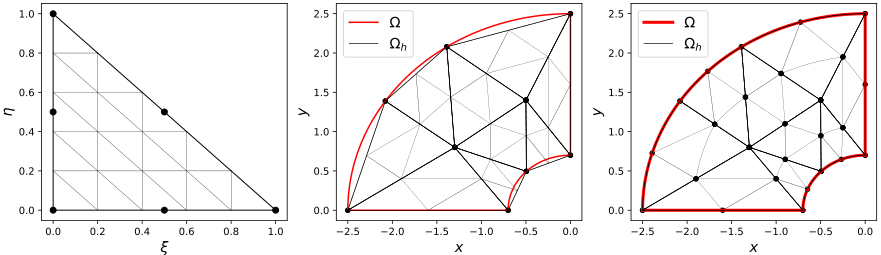
\includegraphics[width=1.\textwidth]{standart_quad_lin_example}
	\caption{Пример аппроксимации и разбиения области \(\Omega\) (<<линейные>> и <<квадратичные>> ячейки)}
	\label{pic:exampleapprox}
\end{figure}

В методе конечных элементов решение системы уравнений~(\ref{eq:generalPDE}) ищется в пространстве базисных функций, или функций формы, а не в физическом пространстве. Решение в каждой ячейке сетки представляется в виде линейной комбинации базисных функций \(\varphi_m(\mathbf x)\):
\begin{equation}\label{eq:Ureconstr}
\mathbf U(\mathbf x, t)\biggm|_{\mathbf{x} \in K_{ie}} = \sum\limits_{m=1}^{K_f} \mathbf u_m(t)\, \varphi_m(\mathbf x),
\end{equation}
где \(\mathbf u_m\) "--- коэффициенты этого разложения, которые являются основными неизвестными величинами в методе конечных элементов.

В данной работе в качестве базисных функций рассматриваются полиномы. Набор функций \(\varphi_m (\mathbf x),~m=\overline{1, K_f}\) образует базис в пространстве полиномов от трёх пространственных координат \((x, y, z)\) степени \(K\). В случае, когда решение уравнения~(\ref{eq:generalPDE}) непрерывно, использование мономов степени \(K\) является необходимым условием для достижения \((K+1)\)-го порядка точности "--- порядка сходимости численного решения при измельчении ячеек сетки. Количество базисных функций \(K_f\) связано с \(K\) соотношением:
\[
K_f = \frac{(K+1) (K+2) (K+3)}{6}.
\]

Существует несколько различных способов определения коэффициентов \(\mathbf u_m\). В методе Галёркина для этого каждое уравнение системы~(\ref{eq:generalPDE}) умножается на базисные функции и интегрируется по контрольному объёму \(\Theta\):
\begin{equation}\label{eq:intPDE}
\iiint\limits_{\Theta} \left(\frac{\partial\mathbf U}{\partial t} + \nabla\cdot \mathbf F\right) \varphi_m(\mathbf x)\: \mathrm d\mathbf x = \iiint\limits_{\Theta} \mathbf S\,\varphi_m(\mathbf x)\: \mathrm d\mathbf x,\quad m = \overline{1, K_f}.
\end{equation}
Подставив разложения~(\ref{eq:Ureconstr}) в соотношения~(\ref{eq:intPDE}) и расписав аппроксимации всех интегралов, получим систему из \(K_f\) уравнений для нахождения \(\mathbf u_m\).

В методе Галёркина с разрывными базисными функциями (РМГ, англ. \textenglish{DG~--- Discontinuous Galerkin}) в разных ячейках используются различные разложения вида (\ref{eq:Ureconstr}), поэтому на гранях ячеек зависимость \(\mathbf U(\mathbf x)\) является, вообще говоря, разрывной. В качестве \(\Theta\) в (\ref{eq:intPDE}) используется объём отдельной ячейки \(K_{ie}\). Таким образом, (\ref{eq:intPDE}) превращается в систему уравнений для нахождения коэффициентов \(\mathbf u_m\) в каждой ячейке. Для консервативности метода "--- выполнения глобальных законов сохранения "--- необходимо, чтобы потоки через общую грань двух соседних ячеек были одинаковы при записи уравнений баланса в каждой из этих ячеек. Так как разложения (\ref{eq:Ureconstr}) в соседних ячейках различны, то потоки через общую грань должны вычисляться по особой процедуре.

Вначале применим к уравнению (\ref{eq:intPDE}) преобразование:
\[
(\nabla\cdot \mathbf F)\, \varphi = \left(\nabla\cdot \mathbf F\,\varphi\right) - \mathbf F\,\nabla\varphi,
\]
а затем "--- формулу Остроградского--Гаусса. В результате получим систему уравнений:
\begin{multline*}
\iiint\limits_{K_{ie}} \frac{\partial \mathbf U}{\partial t} \varphi_m\: \mathrm d\mathbf x + \oint_{\Sigma_{ie}} \left(\mathbf F\cdot \mathbf n\right) \varphi_m\: \mathrm d\Sigma = \\
\iiint\limits_{K_{ie}} \left(\mathbf F\cdot \nabla\varphi_m\right) \mathrm d\mathbf x + \iiint\limits_{K_{ie}} \mathbf S\, \varphi_m\: \mathrm d\mathbf x,\quad m = \overline{1, K_f},
\end{multline*}
где \(K_{ie}\) "--- \(ie\)-я ячейка, \(\Sigma_{ie}\) "--- поверхность \(ie\)-й ячейки, \(\mathbf n\) "--- единичный вектор внешней нормали к элементу поверхности ячейки \(\mathrm d\Sigma\). Вводя следующие обозначения:
\[\begin{aligned}
\mathbf F_n &\equiv \left(\mathbf F\cdot \mathbf n\right) = \mathbf F_x n_x + \mathbf F_y n_y + \mathbf F_z n_z, \\
\mathbf F_m &\equiv \left(\mathbf F\cdot \nabla\varphi_m\right) = \mathbf F_x \frac{\partial \varphi_m}{\partial x} + \mathbf F_y \frac{\partial \varphi_m}{\partial y} + \mathbf F_z \frac{\partial \varphi_m}{\partial z},
\end{aligned}\]
получим более компактную запись:
\begin{multline}\label{eq:PDE:int:sep}
\iiint\limits_{K_{ie}} \frac{\partial \mathbf U}{\partial t} \varphi_m\: \mathrm d\mathbf x + \oint_{\Sigma_{ie}} \mathbf F_n \varphi_m\: \mathrm d\Sigma =\\
\iiint\limits_{K_{ie}} \mathbf F_m\: \mathrm d\mathbf x + \iiint\limits_{K_{ie}} \mathbf S\, \varphi_m\: \mathrm d\mathbf x,\quad m = \overline{1, K_f}.
\end{multline}

Коэффициенты разложения (\ref{eq:Ureconstr}) на известном временном слое обозначим через \(\mathbf u_m^n\), а на неизвестном временном слое "--- \(\mathbf u_m^{n+1}\). Приращения \(\Delta\mathbf u_m\) нужно найти из решения приближенного аналога системы уравнений (\ref{eq:PDE:int:sep}).

В случае, когда базисные функции ортонормированы, используя соотношения (\ref{eq:Ureconstr}), можно переписать систему (\ref{eq:PDE:int:sep}) в виде:
\begin{equation}\label{eq:ODE:dudt}
\frac{\mathrm d\mathbf u_m}{\mathrm d t} = \mathbf R_m,\quad m = \overline{1, K_f},
\end{equation}
где невязка \(\mathbf R_m\) включает интегралы по поверхности и объёму ячейки:
\begin{equation}\label{eq:R}
\mathbf R_m = -\oint_{\Sigma_{ie}} \mathbf F_n \varphi_m\: \mathrm d\Sigma + \iiint\limits_{K_{ie}} \mathbf F_m\: \mathrm d\mathbf x + \iiint\limits_{K_{ie}} \mathbf S\, \varphi_m\: \mathrm d\mathbf x,\quad m = \overline{1, K_f}.
\end{equation}

Таким образом, для нахождения коэффициентов разложения решения в каждой ячейке, необходимы способы вычисления объёмных и поверхностных интегралов.



%%================================
\section{Преобразования координат} \label{sect:transform}
%%================================

Элементы~\(K_{ie}\), на которые разбивается область~\(\Omega_h\), вообще говоря, могут быть произвольными. Однако вычисление интегралов по произвольным ячейкам "--- практически невыполнимая задача. Поэтому вводятся стандартные элементы, для которых известны методы получения точных значений интегралов от полиномов заданной степени. В качестве стандартных элементов используются симметричные фигуры, такие, как куб, квадрат, трёхмерный и двумерный симплексы. Эти элементы, в свою очередь, отображаются в физическое пространство, используя преобразования координат: линейные или квадратичные. Отображение из локального пространства элемента в физическое записывается в виде:
\begin{equation}\label{eq:gentransform}
\left\{\begin{array}{l}
x = x (\xi, \eta, \zeta), \\
y = y (\xi, \eta, \zeta), \\
z = z (\xi, \eta, \zeta), \\
\end{array}\right.\quad \xi, \eta, \zeta \in \hat \Omega.
\end{equation}
Для вычисления поверхностных интегралов по граням ячейки используется параметризация поверхности:
\begin{equation}\label{eq:genparam}
\left\{\begin{array}{l}
x = x (\xi, \eta), \\
y = y (\xi, \eta), \\
z = z (\xi, \eta), \\
\end{array}\right.\quad \xi, \eta \in \hat S.
\end{equation}

Преобразование~(\ref{eq:gentransform}) должно быть симметричным относительно переменных \(\xi\), \(\eta\) и \(\zeta\). При этом преобразования для каждой грани элемента не должны зависеть от координат остальных его вершин, чтобы соседние ячейки соприкасались по граням, т.\,е. чтобы не было <<нахлёстов>> элементов и <<дырок>> между ними.

В данной работе используются преобразования, которые могут быть записаны в следующем виде:
\begin{equation}\label{eq:transform3d}
\newcommand{\pat}[1]{{#1} = \sum_{i=1}^n {#1}_i N_i(\xi, \eta, \zeta)}
\left\{\begin{array}{l}
\pat{x}, \\
\pat{y}, \\
\pat{z}, \\
\end{array}\right.\quad \xi, \eta, \zeta \in \hat \Omega,
\end{equation}
\begin{equation}\label{eq:transform2d}
\newcommand{\pat}[1]{{#1} = \sum_{i=1}^m {#1}_i N_i(\xi, \eta)}
\left\{\begin{array}{l}
\pat{x}, \\
\pat{y}, \\
\pat{z}, \\
\end{array}\right.\quad \xi, \eta \in \hat S,
\end{equation}
где \((x_i, y_i, z_i)\) "--- координаты \(i\)-го узла в физическом пространстве, \(N_i\) "--- функция формы, равная единице в \(i\)-ом узле и нулю в других узлах стандартного элемента.

В работе рассматриваются два семейства конечных элементов: <<линейные>> и <<квадратичные>>. Тип элемента определяется количеством узловых точек на рёбрах. Так, в случае <<линейных>> элементов, количество узлов на каждом ребре ячейки равно двум. Для аппроксимации сложной геометрии небольшим количеством элементов простых <<линейных>> многогранников уже не достаточно. Возникает необходимость вводить <<квадратичные>> элементы, каждое ребро которых представлено тремя узловыми точками~(рис.~\ref{pic:exampleapprox}).

В следующих подразделах выписаны функции формы \(N_i\) для гексаэдров и тетраэдров, подробный вывод которых описан в~\cite{Zienkiewicz:2000:en}.



%%====================
\subsection{Гексаэдры}\label{subsect:hexatransform}
%%====================

\begin{figure}[h]
	{\centering
		\hfill
		\subbottom[Локальное пространство гексаэдра\label{pic:standarthexa}]{
			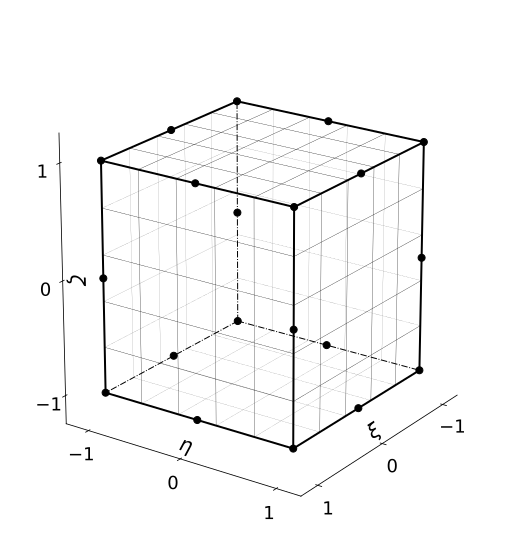
\includegraphics[width=0.48\textwidth]{standart_hexa}}
		\hfill
		\subbottom[Физическое пространство\label{pic:transformedhexa}]{
			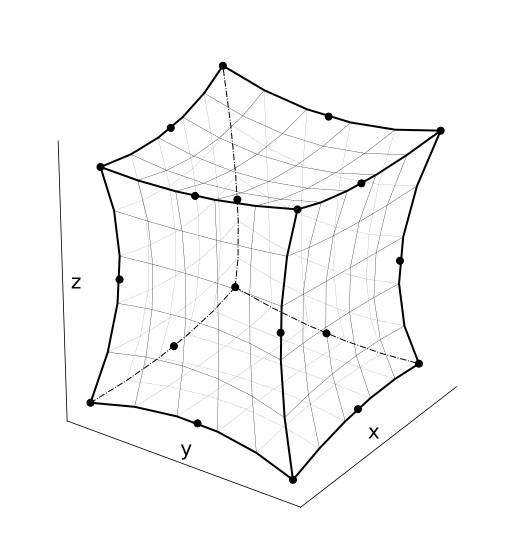
\includegraphics[width=0.48\textwidth]{transformed_hexa}}
		\hfill
	}
	\caption{Стандартный гексаэдр и его отображение в физическое пространство}
	\label{pic:hexatransform}
\end{figure}

Функции формы для <<линейных>> шестигранников имеют следующий вид:
\begin{equation}\label{eq:tr:hexa:lin}
N_i = \frac{1}{8} (1 + \xi_i \xi) (1 + \eta_i \eta) (1 + \zeta_i \zeta),
\end{equation}
где \((\xi_i, \eta_i, \zeta_i)\) "--- координаты i-й вершины <<стандартного>> шестигранника. В данной работе <<стандартный>> шестигранник представлен как куб с вершинами в точках \( \xi = \pm 1,\;\eta = \pm 1,\;\zeta = \pm 1\), как показано на рис. \ref{pic:standarthexa}.

На практике для представления <<квадратичных>> шестигранников часто используют так называемые <<серендиповы>> (serendipity) преобразования~\cite{Zienkiewicz:2000:en}. Они хороши тем, что используют информацию только о гранях ячейки вплоть до <<кубических элементов>>. Пример <<квадратичного>> гексаэдра в физическом пространстве показан на~рис.~\ref{pic:transformedhexa}. Функции формы <<квадратичных>> шестигранников имеют следующий вид:
\begin{itemize}
	\item для угловых узлов:
	\begin{multline}\label{eq:tr:hexa:quad}
	N_i = \frac{1}{8} (1 + \xi_i \xi) (1 + \eta_i \eta) (1 + \zeta_i \zeta)(\xi_i \xi + \eta_i \eta + \zeta_i \zeta - 2), \\
	\xi_i = \pm 1,\; \eta_i = \pm 1,\; \zeta_i = \pm 1,
	\end{multline}
	\item для серединных узлов:
	\begin{multline*}
	N_i = \frac{1}{4} (1 - \xi^2) (1 + \eta_i \eta) (1 + \zeta_i \zeta), \\
	\xi_i = 0,\; \eta_i = \pm 1,\; \zeta_i = \pm 1,\quad \text{и т.д.}
	\end{multline*}
\end{itemize}

Оценка степеней в преобразовании~(\ref{eq:transform3d}) приведена в~табл.~\ref{tab:transformorder:hexa}

\begin{table}[ht]
	\centering
	\caption{Степени полиномов в преобразовании (\ref{eq:transform3d}) для гексаэдров}
	\label{tab:transformorder:hexa}
	\smallskip
	\begin{tabular}{l l c c}
		\toprule
		элемент                           & степень             & преобразования & якобиана \\
		\midrule
		\multirow{2}{*}{<<линейный>>}     & суммарная           & 3              & 5 \\
		                                  & по одной переменной & 1              & 2 \\
		\midrule
		\multirow{2}{*}{<<квадратичный>>} & суммарная           & 4              & 9 \\
                                      & по одной переменной & 2              & 5 \\
		\bottomrule
	\end{tabular}
\end{table}



%%====================
\subsection{Тетраэдры}
%%====================

В отличие от шестигранников, у тетраэдров не все рёбра можно направить вдоль осей координат, что вызывает неудобство. Для компактной записи и для получения функций форм~(\ref{eq:transform3d}) и~(\ref{eq:transform2d}) удобно ввести барицентрические координаты \(L_1, L_2, L_3\) и \(L_4\). Они не являются независимыми и вводятся через систему линейных уравнений:
\begin{equation}\label{eq:barycentricsystem}
\left\{\begin{array}{l}
\xi   = L_1\xi_1   + L_2\xi_2   + L_3\xi_3   + L_4\xi_4,   \\
\eta  = L_1\eta_1  + L_2\eta_2  + L_3\eta_3  + L_4\eta_4,  \\
\zeta = L_1\zeta_1 + L_2\zeta_2 + L_3\zeta_3 + L_4\zeta_4, \\
1 = L_1 + L_2 + L_3 + L_4,
\end{array}\right.
\end{equation}
где \(\xi_i, \eta_i, \zeta_i\) "--- вершины стандартного тетраэдра.

\begin{figure}[h]
	{\centering
		\hfill
		\subbottom[треугольник]{
			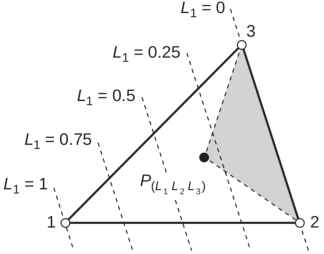
\includegraphics[width=0.5\textwidth]{area_coordinates}}
		\hfill
		\subbottom[тетраэдр]{
			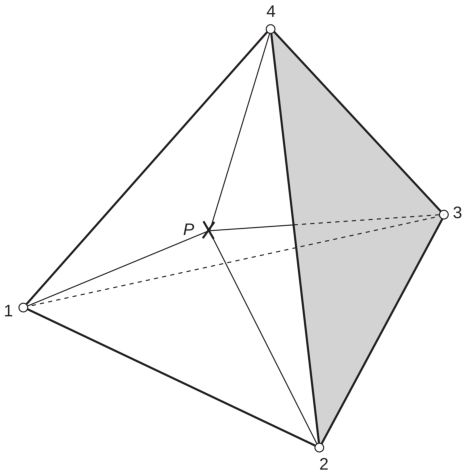
\includegraphics[width=0.4\textwidth]{volume_coordinates}}
		\hfill
	}
	\caption{Барицентрические координаты из~\cite{Zienkiewicz:2000:en}}
	\label{pic:barycentriccoord}
\end{figure}

В~\cite{Zienkiewicz:2000:en} проведен подробный анализ этих уравнений и было показано, что физический смысл барицентрических координат следующий~(рис.~\ref{pic:barycentriccoord}):
\begin{itemize}
	\item в двумерном случае это отношение площадей:
	\[L_1 = \frac{\text{площадь}\; P23}{\text{площадь}\; 123},\quad  \text{и т.д.,}\]
	\item в трёхмерном случае это отношение объёмов:
	\[L_1 = \frac{\text{объём}\; P234}{\text{объём}\; 1234},\quad \text{и т.д.}\]
\end{itemize}

Барицентрические координаты линейно меняются от единицы в соответствующем узле до нуля на противоположной грани. Тогда функции формы линейных элементов следующие~(рис.~\ref{pic:nodesorder:a}):
\begin{equation}\label{eq:tr:tetra:lin}
N_1 = L_1,\quad N_2 = L_2,\quad N_3 = L_3,\quad N_4 = L_4.
\end{equation}

\begin{figure}[t]
	{\centering
		\hfill
		\subbottom[<<линейные>>\label{pic:nodesorder:a}]{
			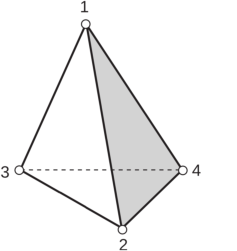
\includegraphics[width=0.45\textwidth]{tetra_4_nodes}}
		\hfill
		\subbottom[<<квадратичные>>\label{pic:nodesorder:b}]{
			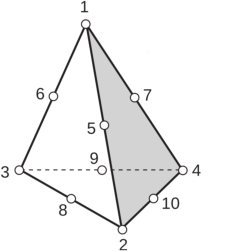
\includegraphics[width=0.45\textwidth]{tetra_10_nodes}}
		\hfill
	}
	\caption{Семейства элементов и расположение узлов из~\cite{Zienkiewicz:2000:en}}
	\label{pic:nodesorder}
\end{figure}

Чтобы получить функции формы элементов более высокого порядка, можно воспользоваться интерполяционными полиномами Лагранжа. Для <<квадратичных>> элементов в~\cite{Zienkiewicz:2000:en} получены следующие функции формы:
\begin{itemize}
	\item для угловых узлов:
	\begin{equation}\label{eq:tr:tetra:quad}
	N_1 = (2L_1 - 1)L_1,\quad \text{и т.д.,}
	\end{equation}
	\item для серединных узлов:
	\[
	N_5 = 4L_1L_2, \quad \text{и т.д.}
	\]
\end{itemize}

В этой работе стандартным тетраэдром является стандартный трёхмерный симплекс: вершины расположены в точках \((0, 0, 0)\), \((1, 0, 0)\), \((0, 1, 0)\), \((0, 0, 1)\)~(рис.~\ref{pic:standartetra}). Тогда решение системы~(\ref{eq:barycentricsystem}) следующее:
\begin{equation}\label{eq:barycentriccoords}
\left\{\begin{array}{l}
L_1 = 1 - \xi - \eta - \zeta, \\
L_2 = \xi, \\
L_3 = \eta, \\
L_4 = \zeta. \\
\end{array}\right.
\end{equation}

Используя соотношения (\ref{eq:tr:tetra:lin}), (\ref{eq:tr:tetra:quad}) и (\ref{eq:barycentriccoords}), в табл.~\ref{tab:transformorder:tetra} получены оценки степени полиномов в преобразовании~(\ref{eq:transform3d}).

\begin{figure}[h]
	{\centering
		\hfill
		\subbottom[Локальное пространство тетраэдра\label{pic:standartetra}]{
			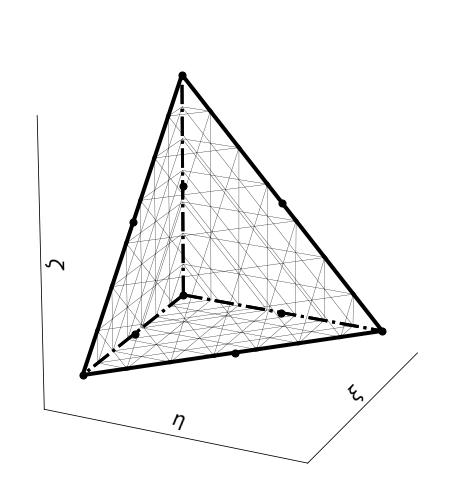
\includegraphics[width=0.48\textwidth]{standart_tetra}}
		\hfill
		\subbottom[Физическое пространство\label{pic:transformedtetra}]{
			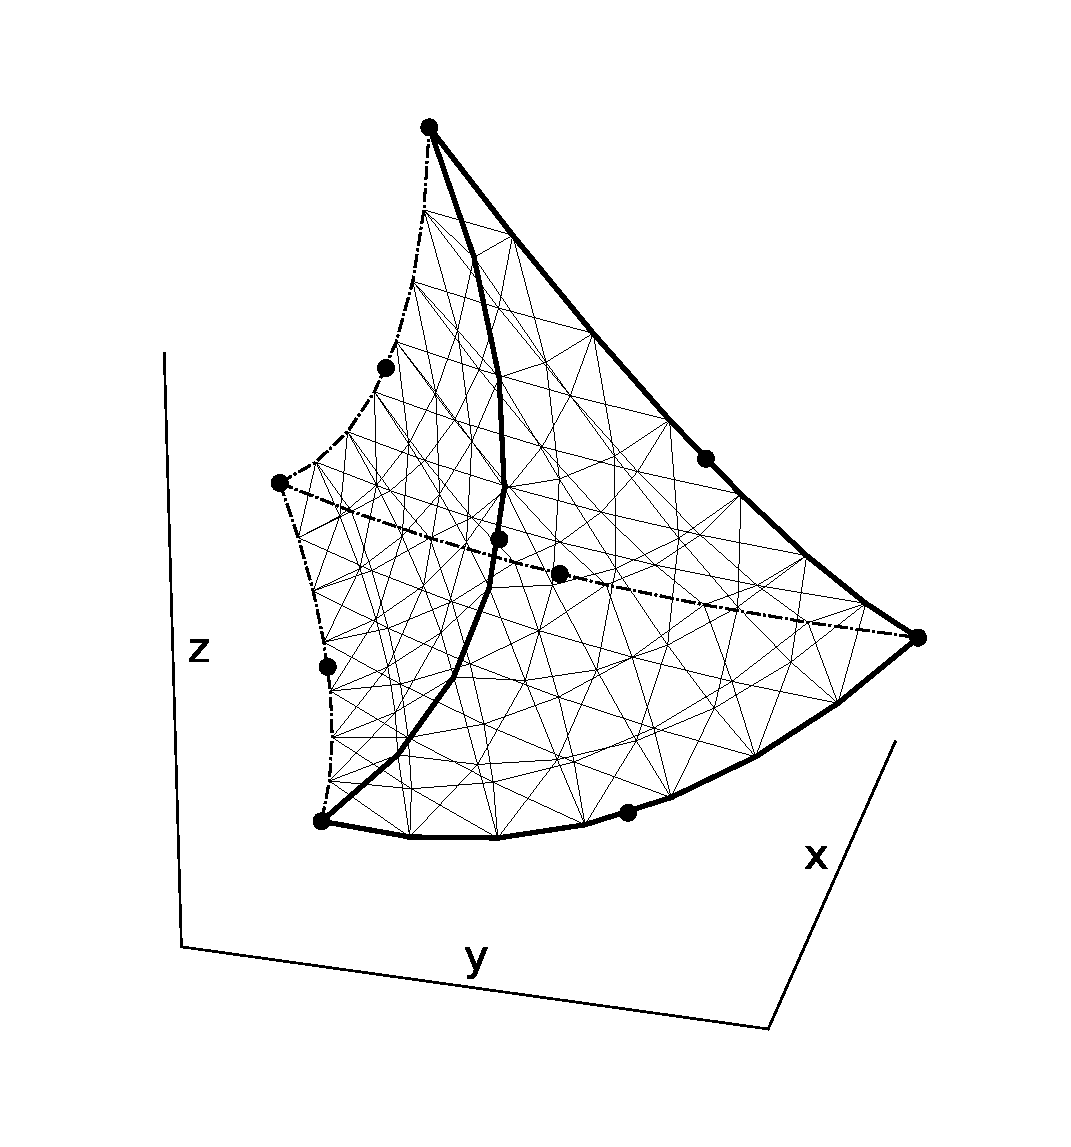
\includegraphics[width=0.48\textwidth]{transformed_tetra}}
		\hfill
	}
	\caption{Стандартный тетраэдр и его отображение в физическое пространство}
	\label{pic:tetratransform}
\end{figure}

\begin{table}[ht]
	\centering
	\caption{Степени полиномов в преобразовании (\ref{eq:transform3d}) для тетраэдров}
	\label{tab:transformorder:tetra}
	\smallskip
	\begin{tabular}{l l c c}
		\toprule
		элемент                           & степень             & преобразования & якобиана \\
		\midrule
		\multirow{2}{*}{<<линейный>>}     & суммарная           & 1              & 0 \\
		                                  & по одной переменной & 1              & 0 \\
		\midrule
		\multirow{2}{*}{<<квадратичный>>} & суммарная           & 2              & 3 \\
		                                  & по одной переменной & 2              & 3 \\
		\bottomrule
	\end{tabular}
\end{table}



%%================================
\subsection{Преобразование граней} \label{subsect:paramfaces}
%%================================

Чтобы провести вычисление поверхностного интеграла по одной из граней элемента~\(K_{ie}\), грань задается в параметрическом виде~(\ref{eq:transform2d})~(рис.~\ref{pic:parametricsurf}). Можно получить систему~(\ref{eq:transform2d}), которая параметрически задаёт конкретную грань, если добавить в~(\ref{eq:transform3d}) определяющее одну из граней соотношение:
\begin{itemize}
	\item в случае гексаэдров:
	\[\xi = \pm 1,\quad \eta = \pm 1,\quad \zeta = \pm 1,\]
	\item в случае тетраэдров:
	\[L_1 = 0,\quad L_2 = 0,\quad L_3 = 0,\quad L_4 = 0.\]
\end{itemize}

\begin{figure}[h]
	{\centering
		\hfill
		\subbottom[Локальное пространство\label{pic:parametricsurf:a}]{
			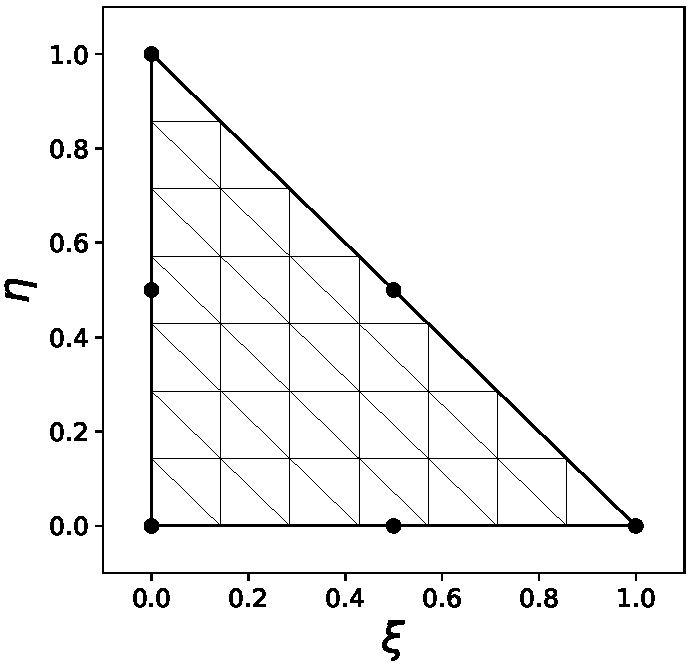
\includegraphics[width=0.4\textwidth]{parametric_surface_standart}}
		\hfill
		\subbottom[Физическое пространство\label{pic:parametricsurf:b}]{
			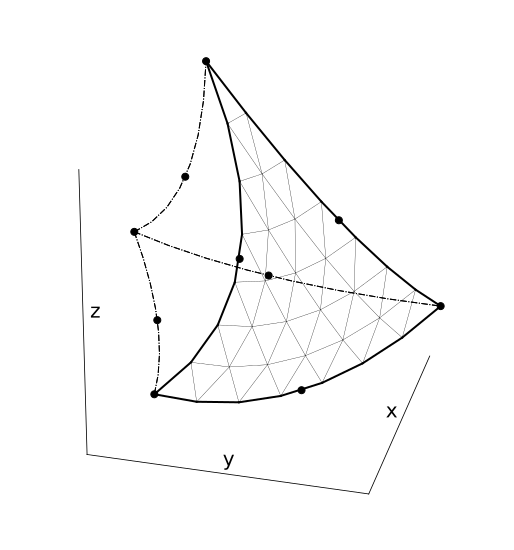
\includegraphics[width=0.5\textwidth]{parametric_surface_real}}
		\hfill
	}
	\caption{Пример параметрического задания грани}
	\label{pic:parametricsurf}
\end{figure}

Чтобы оценить степень подынтегрального выражения, необходимо определить степени полиномов в векторе
\begin{equation}\label{eq:normal}
\mathbf J(\xi, \eta) =
\begin{pmatrix}
\pfrac{x}{\xi} \\[1ex]
\pfrac{y}{\xi} \\[1ex]
\pfrac{z}{\xi} \\
\end{pmatrix}
\times
\begin{pmatrix}
\pfrac{x}{\eta} \\[1ex]
\pfrac{y}{\eta} \\[1ex]
\pfrac{z}{\eta} \\
\end{pmatrix}.
\end{equation}
Оценка степеней полиномов при параметрическом задании граней для гексаэдров приведена в~табл.~\ref{tab:paramorder:hexa}, а для тетраэдров в~табл.~\ref{tab:paramorder:tetra}, где за~\(\mathrm J_{x,y,z}(\xi, \eta)\) обозначен любой элемент вектора~\(\mathbf J\).

\begin{table}[h]
	\centering
	\caption{Степени полиномов при параметрическом задании граней (\ref{eq:transform2d}) гексаэдров}
	\label{tab:paramorder:hexa}
	\smallskip
	\begin{tabular}{l l c c}
		\toprule
		элемент                           & степень             & преобразования & \(\mathrm J_{x,y,z}(\xi, \eta)\) \\
		\midrule
		\multirow{2}{*}{<<линейный>>}     & суммарная           & 2              & 1 \\
		                                  & по одной переменной & 1              & 1 \\
		\midrule
		\multirow{2}{*}{<<квадратичный>>} & суммарная           & 3              & 4 \\
		                                  & по одной переменной & 2              & 3 \\
		\bottomrule
	\end{tabular}
\end{table}

\begin{table}[h]
	\centering
	\caption{Степени полиномов при параметрическом задании граней (\ref{eq:transform2d}) тетраэдров}
	\label{tab:paramorder:tetra}
	\smallskip
	\begin{tabular}{l l c c}
		\toprule
		элемент                           & степень             & преобразования & \(\mathrm J_{x,y,z}(\xi, \eta)\) \\
		\midrule
		\multirow{2}{*}{<<линейный>>}     & суммарная           & 1              & 0 \\
		                                  & по одной переменной & 1              & 0 \\
		\midrule
		\multirow{2}{*}{<<квадратичный>>} & суммарная           & 2              & 1 \\
		                                  & по одной переменной & 2              & 1 \\
		\bottomrule
	\end{tabular}
\end{table}



%%==============================
\section{Правила интегрирования}\label{sect:cubatures}
%%==============================

В методе Галёркина с разрывными базисными функциями один из шагов в алгоритме "--- это вычисление поверхностных и объёмных интегралов по ячейкам расчётной области:
\[
\begin{aligned}
\iiint\limits_{K_{ie}}&F(x, y, z)\: \mathrm d\mathbf x,\\
\iint\limits_{\Sigma_{ie}}&\mathbf F(x, y, z)\cdot \mathrm d\mathbf S,
\end{aligned}
\]
где \( K_{ie}\) "--- элементы, на которое было разбито исходное пространство~(см.~\ref{sect:DG}), \(\Sigma_{ie}\) "--- одна из граней \( K_{ie}\). Используя преобразование~(\ref{eq:gentransform}) и параметризацию для граней~(\ref{eq:genparam}), получим:
{
	\newcommand*{\vecxi}{\xi, \eta, \zeta}
	\begin{multline} \label{eq:volumeintegral}
	\iiint\limits_{K_{ie}}F(x, y, z)\: \mathrm d\mathbf x =\\
	\iiint\limits_{\hat\Omega}F\big(x(\vecxi), y(\vecxi), z(\vecxi)\big) \left|\det\mathbf J(\vecxi)\right|\:\mathrm d\xi\,\mathrm d\eta\, \mathrm d\zeta,
	\end{multline}
}
\begin{equation} \label{eq:surfaceintegral}
\iint\limits_{\Sigma_{ie}}\mathbf F(x, y, z)\cdot \mathrm d\mathbf{S} =
\iint\limits_{\hat{S}}\mathbf F(x(\xi, \eta), y(\xi, \eta), z(\xi, \eta))\cdot \mathbf J(\xi, \eta)\: \mathrm d\xi\, \mathrm d\eta,
\end{equation}
где \(\hat S\) "--- стандартный двумерный элемент, \(\mathbf J(\xi, \eta, \zeta)\) "--- матрица Якоби преобразования~(\ref{eq:transform3d}), \(\mathbf J(\xi, \eta)\) определен в~(\ref{eq:normal}).

На каждом элементе~\( K_{ie}\) вводятся базисные функции, на которые раскладывается искомое решение задачи. В данной работе в качестве базисных функций используют полиномы~(см.~раздел~\ref{sect:DG}). Поэтому подынтегральные функции "--- это полиномы некоторой степени.

Оценим степени подынтегральных выражений~(\ref{eq:volumeintegral}) и~(\ref{eq:surfaceintegral}). Обозначим за~\(k_F\) полную степень полинома~\(F\), за~\(k_T\) степень отображения, и за~\(k_J\) степень якобиана отображения. Получим, что
\begin{equation}\label{eq:intdegree}
k = k_F k_T + k_J.
\end{equation}

Для численного одномерного интегрирования используются квадратурные правила. \textit{Квадратурное правило} обычно определяется множеством различных точек \(\bigl\{x_0,\ldots, x_n \bigr\}\) в диапазоне \([-1,\, 1]\) и множеством соответствующих коэффициентов \(\bigl\{\alpha_0,\ldots, \alpha_n \bigr\}\), называемых весами, которые удовлетворяют соотношению:
\begin{equation}\label{eq:quadrule}
\int_{-1}^{1} p_k(x)\: \mathrm dx \; = \; \sum_{i = 0}^{n} \alpha_i p_k(x_i),
\end{equation}
где~\(p_k(x)\) "--- полином степени~\(k\). Порядок точности интегрирования определяется как максимальная степень~\(k\), для которой  выполнено~(\ref{eq:quadrule}).

Примечательно, что в некоторых квадратурных правилах изначально <<фиксируются>> квадратурные точки, что ведет к уменьшению максимально возможного порядка точности. Так, например, в методе трапеций изначально <<фиксируют>> точки \(x_0 = -1\), \(x_1 = 1\), а затем считают соответствующие веса: \(\alpha_0 = \alpha_1 = 1\). В результате метод является точным только для полиномов первой степени. В квадратурах Гаусса же точки не <<фиксируются>>. Как следствие, для того же количества точек получаем 3-й порядок точности. Снижение количества квадратурных точек позволяет ускорить работу численной схемы. Поэтому целесообразней использовать именно квадратуры Гаусса для одномерного интегрирования.

Стоит отметить, что квадратуры Гаусса можно вывести для любого порядка точности путём нахождения нулей полиномов Лежандра. Для~\(N\) точек максимальная степень подынтегрального полинома, для которого выполнено~(\ref{eq:quadrule}), равна \(2N - 1\).

В многомерном случае в определении~(\ref{eq:quadrule}) \(x\) заменяется на вектор~\(\mathbf x\), а область интегрирования на некоторый элемент, по которому необходимо проводить интегрирование. Элемент, вообще говоря, может быть произвольным. В данной работе рассматриваются два таких элемента "--- гексаэдр и тетраэдр.

Отмечу, что в методе Галёркина с разрывными базисными функциями подынтегральные выражения в объёмном интеграле "--- это полиномы степени \(k_F = 2K\), а в поверхностном "--- полиномы степени \(k_F = 2K + 1\), где \(K\) "--- это степень базисных функций, см. раздел~\ref{sect:DG} и~\cite{Podaruev:2017}.



%%====================
\subsection{Гексаэдры}
%%====================

В таблицах~\ref{tab:integrationorder:hexa} и~\ref{tab:integrationparam:hexa} приведены степени подынтегральных выражений в объёмном~(\ref{eq:volumeintegral}) и поверхностном~(\ref{eq:surfaceintegral}) интегралах.

\begin{table}[h]
	\centering
	\caption{Степени подынтегрального выражения в интеграле по объёму (\ref{eq:volumeintegral})}
	\label{tab:integrationorder:hexa}
	\smallskip
	\begin{tabular}{l l c}
		\toprule
		элемент                                    & степень             & \\
		\midrule
		\multirow{2}{*}{<<линейный>> гексаэдр}     & суммарная           & \(3k_F + 5\) \\
		                                           & по одной переменной & \( k_F + 2\) \\
		\midrule
		\multirow{2}{*}{<<квадратичный>> гексаэдр} & суммарная           & \(4k_F + 9\) \\
		                                           & по одной переменной & \(2k_F + 5\) \\
		\bottomrule
	\end{tabular}
\end{table}

\begin{table}[h]
	\centering
	\caption{Степени подынтегрального выражения в поверхностном интеграле (\ref{eq:surfaceintegral})}
	\label{tab:integrationparam:hexa}
	\smallskip
	\begin{tabular}{l l c}
		\toprule
		элемент                                            & степень             & \\
		\midrule
		\multirow{2}{*}{грань <<линейного>> гексаэдра}     & суммарная           & \(2k_F + 1\) \\
		                                                   & по одной переменной & \( k_F + 1\) \\
		\midrule
		\multirow{2}{*}{грань <<квадратичного>> гексаэдра} & суммарная           & \(3k_F + 4\) \\
		                                                   & по одной переменной & \(2k_F + 3\) \\
		\bottomrule
	\end{tabular}
\end{table}

В случае шестигранников и квадратов, квадратурные правила могут быть получены из одномерных квадратур Гаусса~\cite{Tesini:2008:en}. Область интегрирования "--- стандартный шестигранник: \(\hat\Omega = [-1,\, 1]^3\). Рассмотрим интегрирование функции \(Q_k = \sum_{i, j, h = 0}^k c_{ijh}\xi^i\eta^j\zeta^h\):
\[
\newcommand{\cubature}[3]{\sum_{#1=1}^{N} \alpha_#1 {#2}^#3_#1}
\begin{aligned}
\iiint\limits_{\hat\Omega} Q_k\: \mathrm d\Omega &=  \sum_{i, j, h = 0}^k c_{ijh} \int_{-1}^{1} \int_{-1}^{1} \int_{-1}^{1} \xi^i \eta^j \zeta^h \:d\xi\:d\eta\:d\zeta = \\
&=	\sum_{i, j, h = 0}^k c_{ijh} \int_{-1}^{1} \xi^i\: \mathrm d\xi \int_{-1}^{1} \eta^j\: \mathrm d\eta \int_{-1}^{1} \zeta^h\: \mathrm d\zeta = \\
&= \sum_{i, j, h = 0}^k c_{ijh} (\cubature{p}{\xi}{i})(\cubature{m}{\eta}{j})(\cubature{n}{\zeta}{h}) = \\
&= \sum_{p, m, n = 1}^N \alpha_p\alpha_m\alpha_n Q_k(\xi_p, \eta_m, \zeta_n),
\end{aligned}
\]
где \(N\) "--- количество квадратурных точек, необходимых для интегрирования полинома максимально \(k\)-й степени, \(\alpha_i\) "--- вес для соответствующей квадратурной точки~(\ref{eq:quadrule}). Таким образом, используя квадратуры Гаусса, можно получить правила интегрирования произвольной точности по кубу. В двумерном случае вывод аналогичный. Графическое изображение кубатурных точек в случае квадрата приведено на рис.~\ref{pic:cubature_rect}.

\begin{figure}[h]
	\centering
	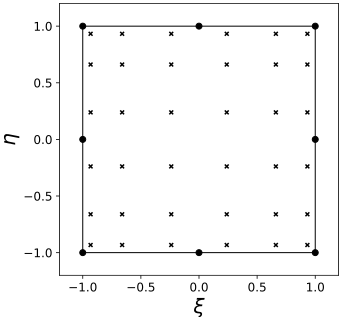
\includegraphics[width=0.49\textwidth]{cubature_rule_6}
	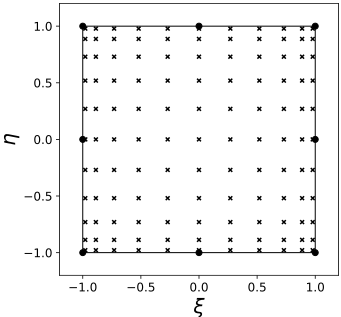
\includegraphics[width=0.49\textwidth]{cubature_rule_11}
	\caption{ Кубатурные точки для квадрата, \(N = 6\) и \(N = 11\)}
	\label{pic:cubature_rect}
\end{figure}

Посчитаем в случае куба для заданной степени \(\text{deg}_{\xi, \eta, \zeta}\) по \(\xi, \eta, \zeta\) количество точек \(N_{\text{cube}}\) и \(N_{\text{square}}\), необходимых для точного интегрирования полинома:
\[
\begin{aligned}
2&N-1 = \text{deg}_\xi\\
&N = \left\lceil \frac{\text{deg}_\xi + 1}{2} \right\rceil \\
&N_{\text{square}} = \left\lceil \frac{\text{deg}_{\xi, \eta} + 1}{2} \right\rceil^2 \\
&N_{\text{cube}} = \left\lceil \frac{\text{deg}_{\xi, \eta, \zeta} + 1}{2} \right\rceil^3
\end{aligned}
\]
Например, для интегрирования по кубу полиномов 9-й степени по \(\xi, \eta, \zeta\) (суммарная степень при этом может быть 27) получаем 125 точек.

Заметим, что, несмотря на высокие суммарные степени полиномов в подынтегральном выражении (см.~табл.~ \ref{tab:integrationorder:hexa} и~\ref{tab:integrationparam:hexa}), каждая переменная в них входит в значительно меньшей степени. Это позволяет снизить количество точек в квадратурных правилах, построенных как декартово произведение одномерных правил.


Рассмотрим теперь интегрирование по объёму и по поверхности одной из грани элемента~\(K_{ie}\):
{
\newcommand*{\vecxi}{\xi, \eta, \zeta}
\newcommand*{\vecxiind}[3]{\xi_#1, \eta_#2, \zeta_#3}
\begin{multline*}
	\iiint\limits_{K_{ie}}F(x, y, z)\: \mathrm d\mathbf x = \iiint\limits_{\hat\Omega}\hat F(\vecxi)\:\mathrm d\xi\,\mathrm d\eta\, \mathrm d\zeta, = \\
	\iiint\limits_{\hat\Omega}F\big(x(\vecxi), y(\vecxi), z(\vecxi)\big) \left|\det\mathbf J(\vecxi)\right|\:\mathrm d\xi\,\mathrm d\eta\, \mathrm d\zeta, = \\
	\sum_{p, m, n = 1}^N \alpha_p\alpha_m\alpha_n F\big(x(\vecxiind{p}{m}{n}), y(\vecxiind{p}{m}{n}), z(\vecxiind{p}{m}{n})\big) \left|\det\mathbf J(\vecxiind{p}{m}{n})\right|,
\end{multline*}
}
\begin{multline*}
\iint\limits_{\Sigma_{ie}}\mathbf F(x, y, z)\cdot \mathrm d\mathbf{S} =
\iint\limits_{\hat{S}}\mathbf F(x(\xi, \eta), y(\xi, \eta), z(\xi, \eta))\cdot \mathbf J(\xi, \eta)\: \mathrm d\xi\, \mathrm d\eta = \\
\sum_{p, m = 1}^M \alpha_p\alpha_m \mathbf F\big(x(s\xi_p, \eta_m), y(\xi_p, \eta_m), z(\xi_p, \eta_m)\big) \cdot \mathbf J(\xi_p, \eta_m),
\end{multline*}
где \(\alpha_i\) "--- вес для соответствующей квадратурной точки (\ref{eq:quadrule}), \(N, M\) "--- количество квадратурных точек в методе Гаусса.



%%====================
\subsection{Тетраэдры} \label{subsect:tetrarules}
%%====================

Используя соотношение~(\ref{eq:intdegree}) и результаты оценки степеней преобразования для тетраэдра из~табл.~\ref{tab:transformorder:tetra}, в таблицах~\ref{tab:integrationorder:tetra} и~\ref{tab:integrationparam:tetra} получены степени подынтегральных выражений в объёмном~(\ref{eq:volumeintegral}) и поверхностном~(\ref{eq:surfaceintegral}) интегралах.

\begin{table}[h]
	\centering
	\caption{Степени подынтегрального выражения в интеграле по объёму (\ref{eq:volumeintegral})}
	\label{tab:integrationorder:tetra}
	\smallskip
	\begin{tabular}{l l c}
		\toprule
		элемент                                    & \multicolumn{2}{l}{степень} \\
		\midrule
		\multirow{2}{*}{<<линейный>> тетраэдр}     & суммарная           & \(k_F\) \\
		                                           & по одной переменной & \(k_F\) \\
		\midrule
		\multirow{2}{*}{<<квадратичный>> тетраэдр} & суммарная           & \(2k_F + 3\) \\
		                                           & по одной переменной & \(2k_F + 3\) \\
		\bottomrule
	\end{tabular}
\end{table}

\begin{table}[h]
	\centering
	\caption{Степени подынтегрального выражения в поверхностном интеграле (\ref{eq:surfaceintegral})}
	\label{tab:integrationparam:tetra}
	\smallskip
	\begin{tabular}{l l c}
		\toprule
		элемент & \multicolumn{2}{l}{степень} \\
		\midrule
		\multirow{2}{*}{грань <<линейного>> тетраэдра}     & суммарная           & \(k_F\) \\
		                                                   & по одной переменной & \(k_F\) \\
		\midrule
		\multirow{2}{*}{грань <<квадратичного>> тетраэдра} & суммарная           & \(2k_F + 1\) \\
		                                                   & по одной переменной & \(2k_F + 1\) \\
		\bottomrule
	\end{tabular}
\end{table}

В случае тетраэдров и треугольников получение кубатурных правил сложнее. Можно, впрочем, используя кубатурные правила для гексаэдров, получить кубатурные правила для тетраэдров с помощью преобразования координат. В качестве примера получим кубатурные правила для треугольника. Воспользуемся уже полученными формулами для линейного преобразования гексаэдра~(\ref{eq:tr:hexa:lin}) (\(\zeta \equiv 1\)) и преобразуем квадрат в треугольник, совместив верхние вершины, как показано на~рис.~\ref{pic:cub:tri:first}:
\begin{equation}\label{eq:totri}
\left\{\begin{array}{l}
\xi = -\frac{1}{4} (\tilde{\xi}\tilde{\eta} + \tilde{\eta} - \tilde{\xi} - 1), \\
\eta = \frac{1}{2} (\tilde{\eta} + 1). \\
\end{array} \right.
\end{equation}
Якобиан отображения:
\[
\det\mathbf J =
\begin{vmatrix}
\frac{1}{4} (1 - \tilde{\eta}) & \frac{1}{4} (1 - \tilde{\xi}) \\
0 & \frac{1}{2}
\end{vmatrix} = \frac{1}{8} (1 - \tilde{\eta}).
\]

\begin{figure}[h]
	{\centering
		\hfill
		\subbottom[Исходный квадрат\label{pic:cub:tri:first:init}]{
			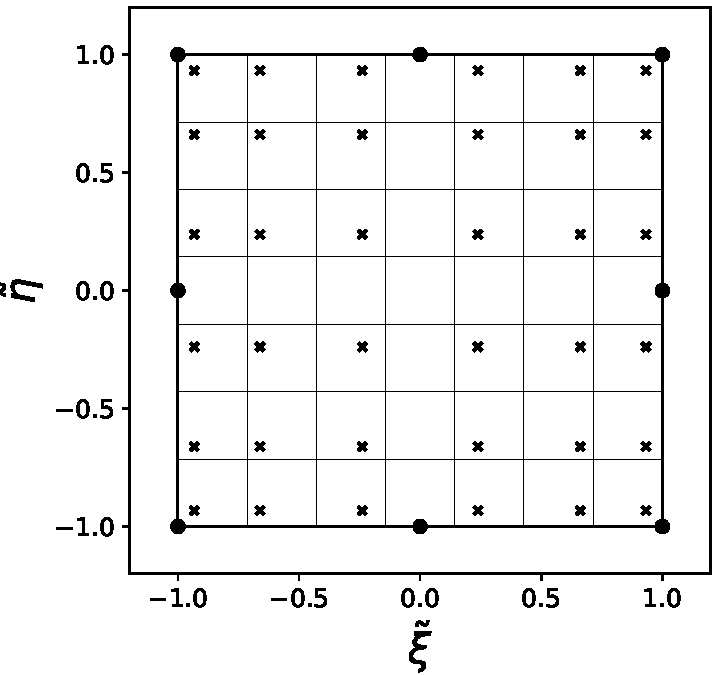
\includegraphics[width=0.48\textwidth]{rect_to_tri_before}}
		\hfill
		\subbottom[Полученный треугольник\label{pic:cub:tri:first:transformed}]{
			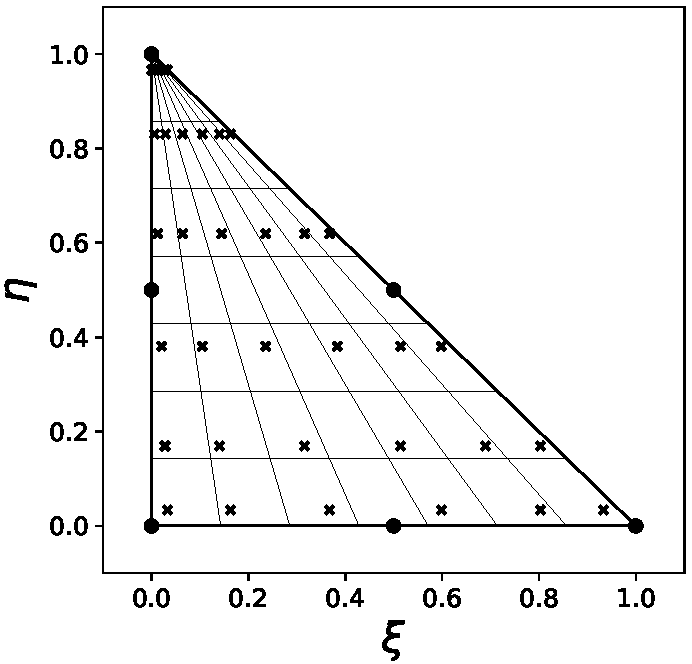
\includegraphics[width=0.48\textwidth]{rect_to_tri_after}}
		\hfill
	}
	\caption{Один из способов получения кубатурных правил}
	\label{pic:cub:tri:first}
\end{figure}

\begin{figure}[h]
	{\centering
		\hfill
		\subbottom[Неоптимальное кубатурное правило, \(N = 16\)]{
			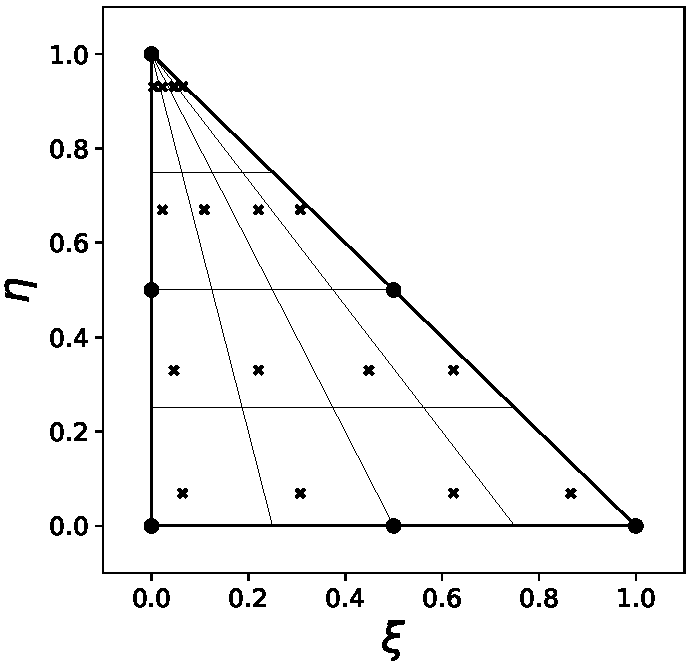
\includegraphics[width=0.48\textwidth]{6_tri_not_opti}}
		\hfill
		\subbottom[Оптимизированное кубатурное правило, \(N = 12\)]{
			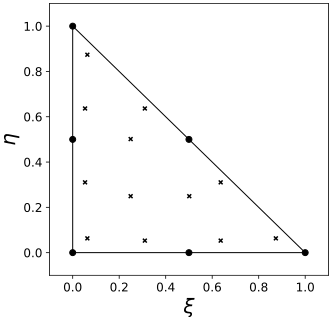
\includegraphics[width=0.48\textwidth]{6_tri_opti}}
		\hfill
	}
	\caption{Сравнение кубатурных правил 6-го порядка для треугольника}
	\label{pic:cub:comparasion}
\end{figure}

Из рис.~\ref{pic:cub:tri:first:transformed} видно, что кубатурные точки получились несимметричными, а также имеется сильное сгущение точек в верхней части треугольника. В численных расчётах это не очень хорошо: мы <<получаем>> много информации из одной части элемента и намного меньше из других. Количество кубатурных точек получилось неоптимальным. Существуют уже готовые симметричные кубатурные правила для тетраэдров и треугольников. Более того, если существующие кубатурные правила не подходят, можно воспользоваться алгоритмом поиска кубатурных правил, см.~\cite{SukumarCubatureRules:2020:en}. Для реализации интегрирования по тетраэдрам в программе~\cite{VolkovA:2010:ru} были использованы уже готовые оптимизированные симметричные кубатурные правила~\cite{CubatureRules}. На рис.~\ref{pic:cub:comparasion} приведены сравнения оптимизированных правил и правил, полученных с использованием (\ref{eq:totri}) для интегрирования по треугольнику полиномов \(\mathbf P (\xi, \eta)\) суммарной степени 6. Видно, что количество кубатурных точек меньше в случае оптимизированных правил.